% -- Document configuration
\documentclass{article}

% -- Input and language settings
% \usepackage[utf8]{inputenc}
\usepackage[spanish]{babel}
\decimalpoint                             % From babel package to use points instead of commas in decimals

% -- Page and line settings
\usepackage{geometry}
\geometry{letterpaper, 
    % margin=2cm, 
    left=3cm, right=3cm,
    top=1.2cm, bottom=1.2cm,
    includefoot, 
    includehead}
\renewcommand{\baselinestretch}{1.2}

% -- Required packages
\usepackage{xcolor}
\usepackage[many]{tcolorbox}
\usepackage{mathtools,amsfonts,amsmath}     % Loads amsmath if not already loaded
\allowdisplaybreaks                         % To allow page breaks if equations are too long
\usepackage[parfill]{parskip}               % No indent and separation lines for paragraphs
\usepackage{cancel}                         % To cancel math terms
\usepackage[shortlabels]{enumitem}          % To handle enumerations
\usepackage{tikz}
\usetikzlibrary{automata, arrows.meta, positioning}
\usepackage[mode=buildnew]{standalone}      % To import figures in standalone files
\usepackage[hidelinks]{hyperref}
\usepackage[spanish]{cleveref}              % To use autocompleted reference labels, language must be change as in babel package
\usepackage{caption}                        % Caption and subcaption to allow subfigures
\usepackage{subcaption}
\usepackage{float}                          % To specify the location of figures
\usepackage{multicol}                       % To use multicolumns
\usepackage[bottom]{footmisc}               % To locate footnotes at the bottom

% -- Title and heading settings
\usepackage{titling}
\usepackage{fancyhdr}
\pagestyle{fancy}

% -- Code and code formatting
\usepackage{minted}                         % To insert code
\usemintedstyle[julia]{gruvbox-light}       % Code theme and language
\definecolor{bg}{rgb}{0.98, 0.97, 0.88}     % Code block background

\usepackage{fontspec}                       % To allow the use of monospace fonts
\setmonofont{JuliaMono}[Path=./codefonts/, Extension=.ttf, UprightFont=*-Regular, ItalicFont=*-RegularItalic, Scale=0.75]

\usepackage{fancyvrb}                       % To change line number font
\renewcommand{\theFancyVerbLine}{\textcolor{gray}{\footnotesize\texttt{\arabic{FancyVerbLine}}}}

\definecolor{light-gray}{gray}{0.95}        % Color, box and style to show small code thingys inside normal text
\newcommand{\code}[1]{\colorbox{light-gray}{\texttt{#1}}}

% -- Bilbiography preferences
\usepackage[square,numbers]{natbib}
\bibliographystyle{unsrt}

% -- Footnotes without numbering
\newcommand\nnfootnote[1]{%
  \begin{NoHyper}
  \renewcommand\thefootnote{}\footnote{#1}%
  \addtocounter{footnote}{-1}%
  \end{NoHyper}
}

% -- Theorems
\newtheorem{theorem}{Theorem}

\lhead{\theinstitution\ -- \thedepartment}
\chead{}
\rhead{Programación para la IA\ -- \thetitle}
\lfoot{}
\cfoot{\thepage}
\rfoot{}

% -- Problem solution
\newenvironment{solution}
{\begin{quote}
\textbf{Solución:}\medskip

}
{

\hfill\rule{0.5\textwidth}{0.5pt}
\end{quote}}

% -- Equation result
\newcommand{\result}[1]
{
\tcbhighmath[colframe=white, colback=gray!15, sharp corners]
{#1}
}

% -- Function definitions
\newcommand{\dprod}[2]{{#1} \cdot {#2}}
\newcommand{\txtgray}[1]{\textcolor{gray}{#1}}

% -- Author information
\title{Actividad 5}
\author{Leonardo Flores Torres}
\newcommand\theinstitution{Universidad Veracruzana}
\newcommand\thedepartment{Inteligencia Artificial}
\newcommand\thecourse{Programación para la Inteligencia Artificial}

% -- Paths
% \newcommand\codelists{../programs/lists.rkt}

% Remove red color boxes of "syntax errors" in minted
\AtBeginEnvironment{minted}{%
  \renewcommand{\fcolorbox}[4][]{#4}}

% -- Document
\begin{document}

\thispagestyle{empty}

%Title
\begin{center}
\textsc{\theinstitution}\\[2mm]

\thedepartment

\rule{0.6\textwidth}{0.5pt}\\[2mm]

\thecourse \\[4mm]

{\Large \textbf{\thetitle}}\\[2mm]

\theauthor \\[2mm]

{\small \today}
\end{center}
\medskip

% -- 
\vspace{1cm}

\textbf{Resolución del problema del viajero utilizando recocido simulado.}

A partir de las coordenadas de las capitales de México, en cada ejecución del algoritmo:
\begin{enumerate}
    \item Dar el valor del número $N$ de ciudades que se utilizarán.
    \item Hacer una selección aleatoria de $N'$ ciudades.
    \item Resolver el problema del viajero para ese conjunto de ciudades empleando el algoritmo de recocido simulado.
    \item Para un número $N'$ de ciudades menor que 10 compare la solución $d_s$ obtenida por recocido simulado con la solución $d^{\star}$ que se genera al computar todas las posibilidades $N'!$ mediante fuerza bruta. La comparación debe realizarse en términos del error en la distancia, $E = |d^{\star} - d_s|$.
    \item Probar con al menos 3 valores distintos de $N$, y donde uno de esos valores sea la totalidad de las ciudades capitales de México.
    \item Mostrar de manera gráfica la solución final obtenida en cada caso.
\end{enumerate}

Este problema, \textit{the travelling salesman problem}, es uno de encontrar la ruta más óptima ¿Pero óptima en qué sentido? La proposición inicial del problema fue el de encontrar la ruta que minimice la distancia al recorrer un conjunto de puntos de interés, aunque podría extenderse este concepto a encontrar la ruta que minimice el tiempo al recorrer estos puntos, o el costo monetario para completar la ruta. Este problema es, en principio, un problema de minimizar una función y la manera de hacerlo es haciendo alusión a un sistema físico.

Primero se podría pensar, y con toda razón, que es un problema de encontrar la combinación del orden en que se visitan estos puntos de interés la cual dé como resultado la distancia más corta de todo el recorrido. Este razonamiento tiene sentido teóricamente pero hay un problema con ello, al aumentar el número $N$ de puntos de interés a visitar el número de combinaciones crece como $N!$. Si en México se quisieran visitar 5 ciudades entonces se tendrían que obtener todas las permutaciones posibles. El número total de permutaciones es igual a
\begin{equation*}
    _{n}{P}_{r} = \frac{n!}{(n - k)!} ,
\end{equation*}
donde $n$ es el tamaño del conjunto, en este caso la cantidad total de puntos de interés, y $k$ es la del tamaño del subconjunto, que corresponde a la cantidad de puntos de interés que sí se van a visitar del total. Si se visitan todos los puntos de interés, entonces $n = k$ y obtenemos que la cantidad total de permutaciones es igual a $_{n}P_{r} = n!$. Si nuestro conjunto es de 5 ciudades, y se visitarán las 5, entonces el total de permutaciones es 120. Si se tienen 10 ciudades y se visitaran todas, entonces el total de permutaciones aumenta a 3628800. Y si fuesen 15, las permutaciones incrementarian a un ridículo total de 1307674368000 ¿Cómo se puede encontrar la mejor ruta con tantas maneras distintas de realizar el recorrido? El problema parece simple de resolver, sí, cuando no se consideran tantos puntos de interés. El trabajo presente apunta a encontrar una solución a esta incógnita tomando a los puntos de interés como las capitales de México siendo un total de 32.

Antes de continuar quisiera mencionar que no fui capaz de realizar el cómputo mediante fuerza bruta considerando el total de capitales lo cuál era de esperarse, ya que computar todas las permutaciones requiere memoria y la librería en \code{julia} disponible para el cómputo de permutaciones depende de la función \code{factorial} la cual tiene una restricción, no puede ser usada para valores mayores a 20. Por lo que \code{factorial(21)} ya no computa.

\begin{figure}[ht!]
    \centering
    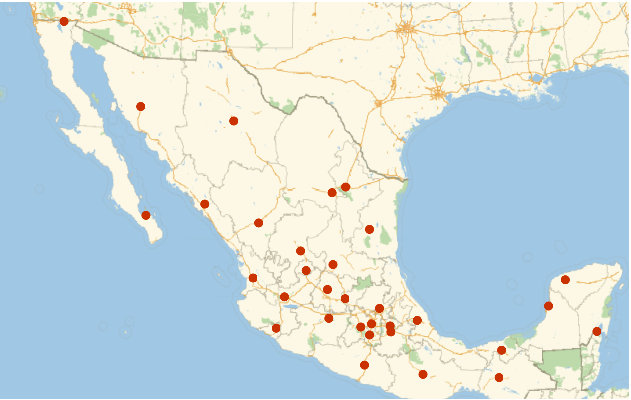
\includegraphics[scale=0.8]{../figures/capital_locations.pdf}
    \caption{Ubicación de las capitales de México.}
    \label{fig:capitales_mexico}
\end{figure}

Las capitales de México se pueden ver ubicadas en la \cref{fig:capitales_mexico} con circulos de color rojo, siendo un total de 32 marcadores. Las coordenadas fueron obtenidas usando GoogleMaps buscando cada ciudad y tomando sus coordenasas aproximadamente en sus centros. Se implementó una función para guardar la información de las capitales, \code{available\_cities}, y usarla posteriormente cuando se necesite hacer una selección aleatoria de las mismas.

Comenzaremos tomando 5 ciudades de manera aleatoria, se mostrarán los nombres de las ciudades seleccionadas (en el orden en que se visitarán) junto con sus latitudes y longitudes correspondientes, como se muestra a continuación:
\begin{minted}[
    frame=none,
    autogobble,
    obeytabs=false,
    breaklines,
    tabsize=4,
    linenos=true,
    baselinestretch=1,
    firstnumber=last,
    bgcolor=bg!70,
    mathescape,
    numberblanklines=false
    ]{julia}
    # Seleccion aleatoria de ciudades
    julia> sample_cities = ts.sample_cities(5);

    # Mostrar ciudades seleccionadas
    julia> map(x -> x.name, sample_cities)
    5-element Vector{String}:
    "oaxaca"
    "saltillo"
    "zacatecas"
    "queretaro"
    "tlaxcala"

    # Mostrar coordenadas de ciudades seleccionadas
    julia> map(x -> (x.lat, x.lon), sample_cities)
    5-element Vector{Tuple{Float64, Float64}}:
    (17.062183511066106, -96.72572385123796)
    (25.425170167352245, -101.00211644466016)
    (22.772858479171045, -102.57341087527752)
    (20.592088731107133, -100.3918227421049)
    (19.314544474512967, -98.23851540921879)
\end{minted}

El mapeo muestra el nombre de las ciudades en el orden en el que se van a visitar, se comienza en Oaxaca y se termina en Tlaxcala. Aunque este es un viaje redondo, esto significa que después de haber llegado a Tlaxcala se debe regresar a Oaxaca nuevamente. En la \cref{fig:trip_cities_05_init} se puede observar el recorrido inicial de esta configuración, 
\begin{figure}[ht!]
    \centering
    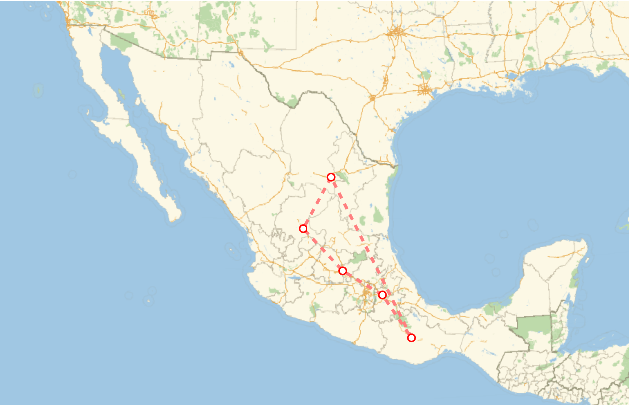
\includegraphics[scale=0.8]{../figures/trip_cities_05_init.pdf}
    \caption{Ruta inicial para cinco capitales comenzando en Oaxaca.}
    \label{fig:trip_cities_05_init}
\end{figure}

El recorrido mostrado en \cref{fig:trip_cities_05_init} es el realizado si se hiciera caso a la selección aleatoria, pero no se desea eso. Primero se calcularán las permutaciones de la selección aleatoria de capitales guardada en \code{sample\_cities}:
\begin{minted}[
    frame=none,
    autogobble,
    obeytabs=false,
    breaklines,
    tabsize=4,
    linenos=true,
    baselinestretch=1,
    firstnumber=last,
    bgcolor=bg!70,
    mathescape,
    numberblanklines=false
    ]{julia}
    # Computando las permutaciones
    julia> path_permutations = ts.brute_force(sample_cities, "geo");

    # Calculando la distancia de cada ruta
    julia> path_permutations_dist = ts.total_distance.(path_permutations, "geo");
\end{minted}

Teniendo las permutaciones se buscará la ruta con la distancia mínima, y también alguna otra ruta cuya distancia sea igual a la mínima, como se muestra a continuación:
\begin{minted}[
    frame=none,
    autogobble,
    obeytabs=false,
    breaklines,
    tabsize=4,
    linenos=true,
    baselinestretch=1,
    firstnumber=last,
    bgcolor=bg!70,
    mathescape,
    numberblanklines=false
    ]{julia}
    # Camino de distancia minima
    julia> min_path = path_permutations[argmin(path_permutations_dist)]

    # Distancia minima
    julia> min_dist = minimum(path_permutations_dist)
    2250.1837692021245

    # Buscando los indices del camino o caminos mas cortos cuya distancia sea igual a la minima encontrada
    julia> optimal_indexes = findall(x -> x == min_dist, path_permutations_dist)
    10-element Vector{Int64}:
    15
    19
    33
    44
    59
    62
    77
    88
    102
    106

    # Encontrando las rutas que coinciden con la distancia minima
    julia> map.(x -> x.name, path_permutations[optimal_indexes])
    10-element Vector{Vector{String}}:
    ["oaxaca", "queretaro", "zacatecas", "saltillo", "tlaxcala"]    # Permutacion optima $\label{line:permutacion_optima_ciudades_5}$
    ["oaxaca", "tlaxcala", "saltillo", "zacatecas", "queretaro"]
    ["saltillo", "zacatecas", "queretaro", "oaxaca", "tlaxcala"]
    ["saltillo", "tlaxcala", "oaxaca", "queretaro", "zacatecas"]
    ["zacatecas", "saltillo", "tlaxcala", "oaxaca", "queretaro"]
    ["zacatecas", "queretaro", "oaxaca", "tlaxcala", "saltillo"]
    ["queretaro", "oaxaca", "tlaxcala", "saltillo", "zacatecas"]
    ["queretaro", "zacatecas", "saltillo", "tlaxcala", "oaxaca"]
    ["tlaxcala", "oaxaca", "queretaro", "zacatecas", "saltillo"]
    ["tlaxcala", "saltillo", "zacatecas", "queretaro", "oaxaca"]
\end{minted}

De esta manera nos hemos asegurado de encontrar todas las ocurrencias donde las distancias de los caminos son iguales al mínimo encontrado. Si no se hubiése hecho así y solamente se hubiera aplicado la función \code{minimum} sí que se habría detectado un mínimo, pero solamente uno. A pesar de que la primera capital en el muestreo aleatorio de capitales fue Oaxaca esto no restringe a que se deba partir de ahí, y también debe recordarse que todas las rutas mostradas con el mismo resultado son rutas de viaje redondo.
\begin{figure}[ht!]
    \centering
    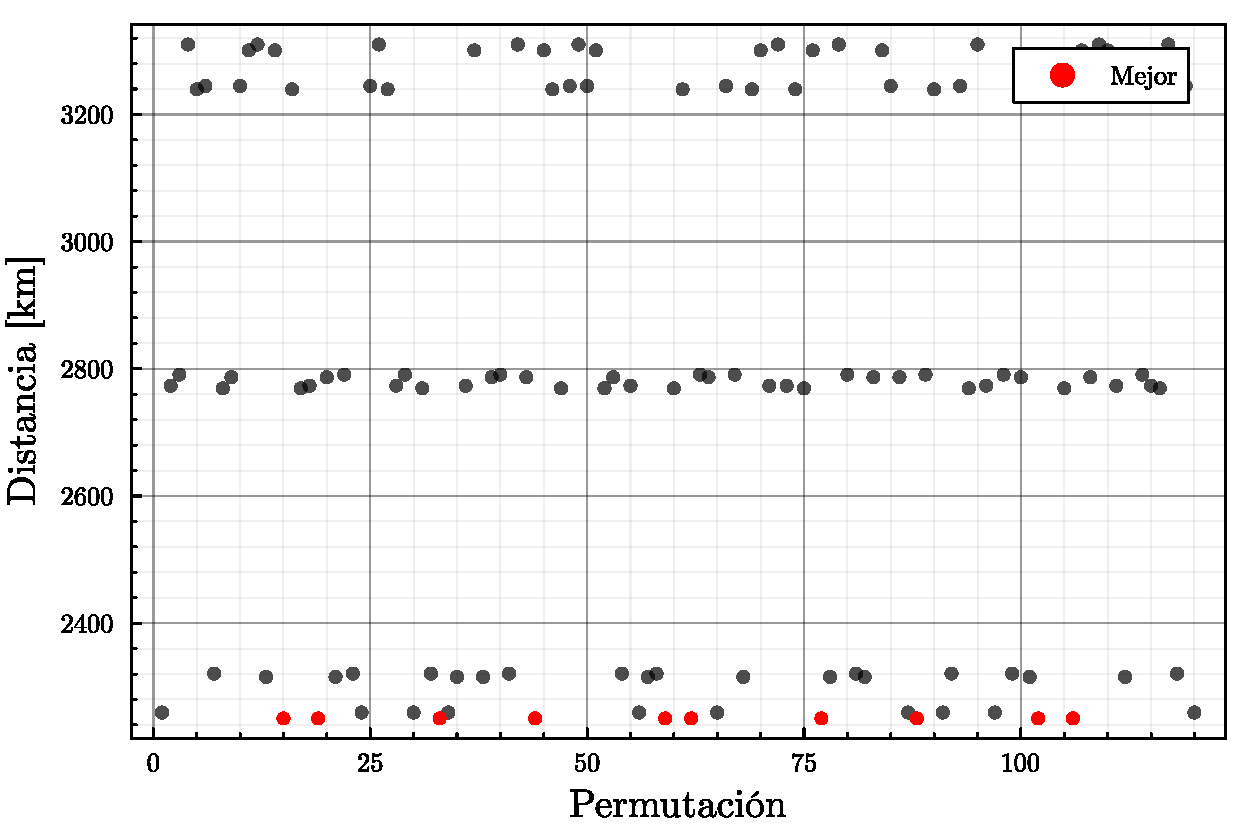
\includegraphics[scale=0.5]{../figures/distances_cities_05_bruteforce.pdf}
    \caption{Distancia por permutación considerando 5 capitales.}
    \label{fig:bruteforce_distances_cities_05}
\end{figure}

De la \cref{fig:bruteforce_distances_cities_05} se puede observar en marcadores rojos aquellas permutaciones con la misma distancia mínima, mientras que los de color grisáceo son rutas menos óptimas. En realidad se podría elegir cualquier ruta de las marcadas en rojo pero para motivos de este trabajo vamos a trabajar con la guardada en \code{min\_path}. El recorrido de esta ruta se puede observar en \cref{fig:bruteforce_path_cities_05}.
\begin{figure}[ht]
    \centering
    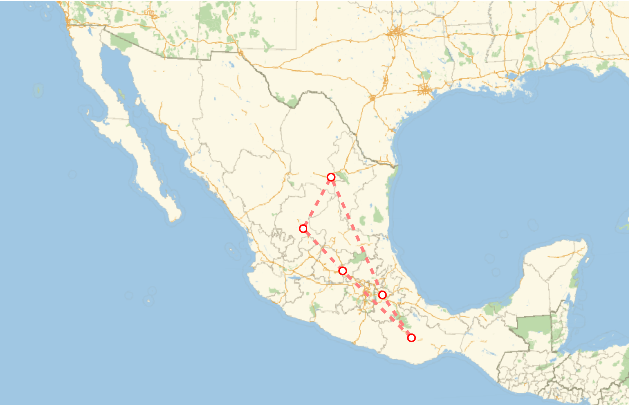
\includegraphics[scale=0.8]{../figures/trip_cities_05_bruteforce.pdf}
    \caption{Ruta óptima para 5 capitales mediante fuerza bruta.}
    \label{fig:bruteforce_path_cities_05}
\end{figure}

Podemos calcular la mejor ruta para esta configuración utilizando el algoritmo de recocido simulado, para esto primero se tiene que dar una suposición inicial que para este caso bien podría coincidir con el orden de las ciudades obtenidas mediantes el muestreo aleatorio. En los casos siguientes se hará una suposición aleatoria inicial del orden de las ciudades para usarlas como entrada en el algoritmo de recocido simulado; aquí se realizará de igual forma.
\begin{minted}[
    frame=none,
    autogobble,
    obeytabs=false,
    breaklines,
    tabsize=4,
    linenos=true,
    baselinestretch=1,
    firstnumber=last,
    bgcolor=bg!70,
    mathescape,
    numberblanklines=false
    ]{julia}
    julia> init_guess_indexes = ts.initial_guess(5)
    5-element Vector{Int64}:
    5
    4
    1
    3
    2

    julia> init_guess = sample_cities[init_guess_indexes]
    5-element Vector{TravellingSalesman.CoordCity}:
    TravellingSalesman.CoordCity("tlaxcala", 19.314544474512967, -98.23851540921879)
    TravellingSalesman.CoordCity("queretaro", 20.592088731107133, -100.3918227421049)
    TravellingSalesman.CoordCity("oaxaca", 17.062183511066106, -96.72572385123796)
    TravellingSalesman.CoordCity("zacatecas", 22.772858479171045, -102.57341087527752)
    TravellingSalesman.CoordCity("saltillo", 25.425170167352245, -101.00211644466016)
\end{minted}

El algoritmo tiene un máximo de iteraciones de $1000$ pero se puede cambiar si así se requiere o desea aunque se agregó un criterio de terminación temprana. Este criterio detiene el algoritmo si detecta que el valor absoluto de la diferencia de distancias entre el recorrido de dos iteraciones consecutivas es menor a un valor de tolerancia, $|d_{i} - d_{i-1}| < \varepsilon$. El punto de hacer esto es aprovechar la naturaleza aleatoria de los cambios de ciudades en la ruta, si dos rutas tienen distancias totales similares o la misma, significa que se ha encontrado la ruta óptima deseada y no es necesario seguir computando las iteraciones precedentes que todavía podrían estar pendientes.
\begin{minted}[
    frame=none,
    autogobble,
    obeytabs=false,
    breaklines,
    tabsize=4,
    linenos=true,
    baselinestretch=1,
    firstnumber=last,
    bgcolor=bg!70,
    mathescape,
    numberblanklines=false
    ]{julia}
    # Aplicacion de recocido simulado al problema del viajero
    julia> best, coords_per_iter, distance_per_iter = ts.simulated_annealing(init_guess, "geo"; init_temp=50, temp_factor=0.99, max_iter=1000, abstol=1E-5)

    # Listado de orden de visita de ciudades por iteracion
    julia> map.(x -> x.name, coords_per_iter)
    5-element Vector{Vector{String}}:
    ["tlaxcala", "queretaro", "oaxaca", "zacatecas", "saltillo"]
    ["zacatecas", "tlaxcala", "oaxaca", "queretaro", "saltillo"]
    ["zacatecas", "oaxaca", "tlaxcala", "queretaro", "saltillo"]
    ["zacatecas", "saltillo", "tlaxcala", "oaxaca", "queretaro"]
    ["oaxaca", "queretaro", "zacatecas", "saltillo", "tlaxcala"]    # Ruta optima $\label{line:ruta_optima_ciudades_5}$

    # Listado del orden de las distancias totales de las rutas encontradas
    julia> distance_per_iter
    5-element Vector{Float64}:
    2769.355722677771
    2315.46679146938
    2320.7163046789665
    2250.1837692021245
    2250.1837692021245    # Distancia de la ruta optima
\end{minted}
Es importante notar que esta ruta mostrada en la línea \ref{line:ruta_optima_ciudades_5} es la misma ruta que la primera listada en la línea \ref{line:permutacion_optima_ciudades_5}, cuando se encontraron todas las permutaciones de las rutas, por lo que la ruta encontrada mediante el algoritmo de recocido simulado será igual a la mostrada en la \cref{fig:bruteforce_path_cities_05}. La última ruta mostrada en el listado de las rutas por iteraciones es la ruta óptima que el algoritmo encuentra, y se guarda en la variable \code{best}. La diferencia de la distancia óptima encontrada por fuerza bruta y la distancia correspondiente a la ruta óptima encontrada por el algoritmo de recocido simulado se muestra en la \cref{fig:delta_distances_cities_05}.
\begin{figure}[ht!]
    \centering
    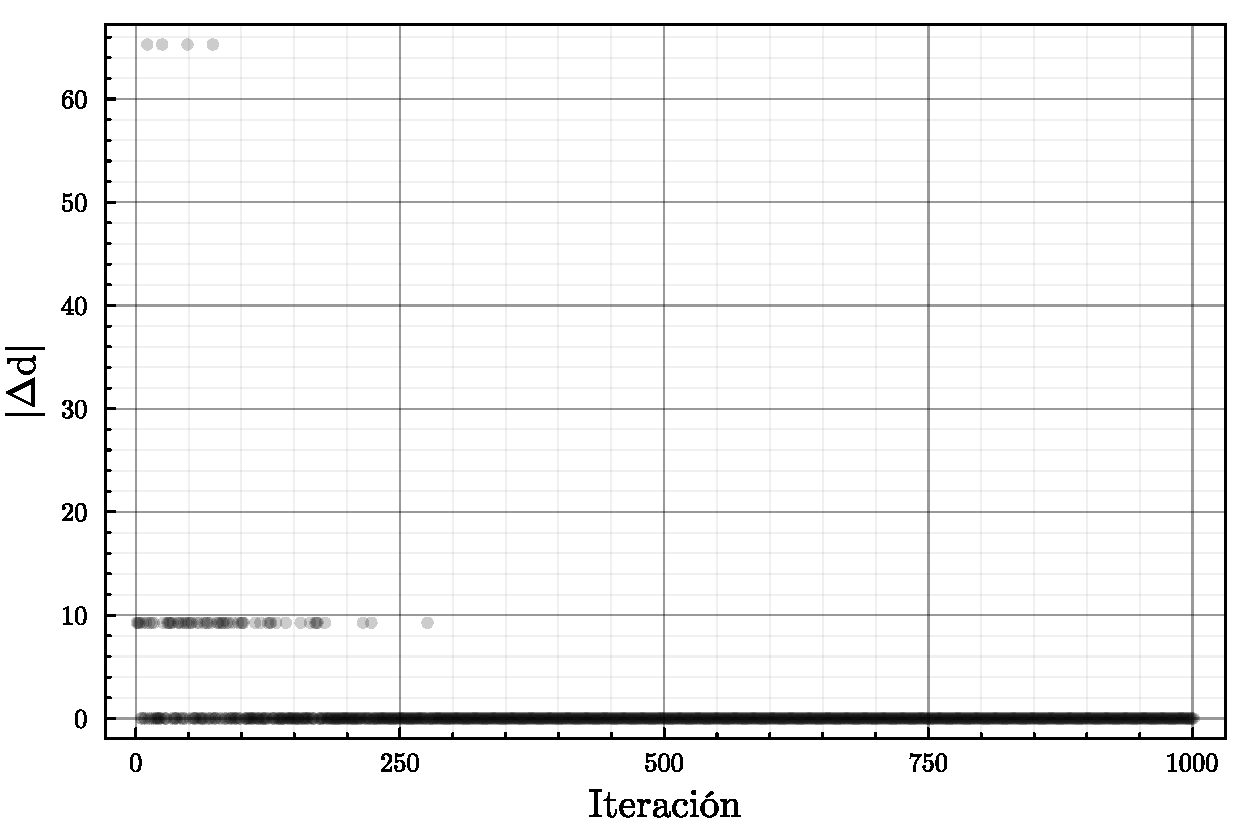
\includegraphics[scale=0.5]{../figures/delta_distances_cities_05.pdf}
    \caption{Diferencia entre la distancia óptima obtenida por fuerza bruta y la mejor distancia obtenida mediante el algoritmo.}
    \label{fig:delta_distances_cities_05}
\end{figure}

Se puede observar que hay muchas iteraciones en las que la configuración de la ruta coincide con alguna ruta óptima, y aproximadamente después de la iteración 250 es que se ha convergido a una ruta óptima ya que no se observan cambios en la diferencia de distancias. Por esto es que se decidió agregar una condición para la terminación temprana del algoritmo de recocido simulado.

Se hubiera deseado tomar un número más grande de ciudades para aplicar la comparación entre el algoritmo de recocido simulado y el método por fuerza bruta pero el número de permutaciones aumenta tanto que en el equipo de cómputo utilizado resulta imposible llegar a casos más grandes. anteriormente se había mencionado el problema con la función \code{factorial}, pero ahora al tratar de computar las permutaciones para 15 y 20 ciudades, la memoria del ordenador fue insuficiente. Ahora que ya se explicó el proceso para encontrar la ruta óptima se procederá a hacer lo mismo tomando un total de 10 ciudades, el muestreo aleatorio de la lista total de capitales y la suposición inicial para el recorrido se muestran a continuación:
\begin{minted}[
    frame=none,
    autogobble,
    obeytabs=false,
    breaklines,
    tabsize=4,
    linenos=true,
    baselinestretch=1,
    firstnumber=last,
    bgcolor=bg!70,
    mathescape,
    numberblanklines=false
    ]{julia}
    julia> sample_cities = ts.sample_cities(10);

    julia> map(x -> x.name, sample_cities)
    10-element Vector{String}:
    "ciudadvictoria"
    "saltillo"
    "villahermosa"
    "durango"
    "zacatecas"
    "aguascalientes"
    "chihuahua"
    "puebla"
    "hermosillo"
    "chetumal"

    julia> init_guess_indexes = ts.initial_guess(10);

    julia> init_guess = sample_cities[init_guess_indexes];

    julia> map(x -> x.name, init_guess)
    10-element Vector{String}:
    "hermosillo"
    "zacatecas"
    "ciudadvictoria"
    "chetumal"
    "durango"
    "villahermosa"
    "aguascalientes"
    "saltillo"
    "puebla"
    "chihuahua"
\end{minted}

El recorrido aleatorio inicial para el caso de las 10 ciudades es el mostrado en la \cref{fig:trip_cities_10_init}. No se espera que el recorrido inicial sea óptimo de ninguna manera ya que el orden se genera de manera aleatoria. Posterior a generar este recorrido aleatorio se deben de calcular las permutaciones de todas las rutas posibles lo cual se hará a continuación:
\begin{figure}[ht!]
    \centering
    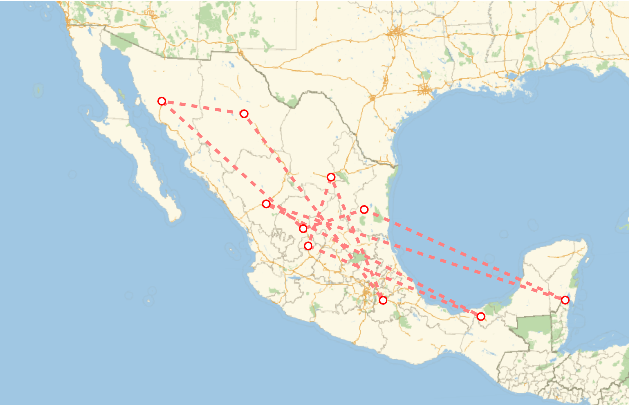
\includegraphics[scale=0.8]{../figures/trip_cities_10_init.pdf}
    \caption{Recorrido aleatorio inicial para un total de 10 ciudades.}
    \label{fig:trip_cities_10_init}
\end{figure}

\begin{minted}[
    frame=none,
    autogobble,
    obeytabs=false,
    breaklines,
    tabsize=4,
    linenos=true,
    baselinestretch=1,
    firstnumber=last,
    bgcolor=bg!70,
    mathescape,
    numberblanklines=false
    ]{julia}
    julia> path_permutations = ts.brute_force(init_guess, "geo");

    julia> path_permutations_dist = ts.total_distance.(path_permutations, "geo");

    julia> min_path = path_permutations[argmin(path_permutations_dist)];

    julia> min_dist = minimum(path_permutations_dist)
    5416.112742134113

    julia> optimal_indexes = findall(x -> x == min_dist, path_permutations_dist)
    11-element Vector{Int64}:
    123655
    353711
    488642
    597881
    1490556
    1516018
    1948927
    2487212
    2633601
    3121779
    3560158

    julia> map.(x -> x.name, path_permutations[optimal_indexes])
    11-element Vector{Vector{String}}:
    ["hermosillo", "durango", "zacatecas", "aguascalientes", "puebla", "villahermosa", "chetumal", "ciudadvictoria", "saltillo", "chihuahua"]    # Permutacion optima
    ["hermosillo", "chihuahua", "saltillo", "ciudadvictoria", "chetumal", "villahermosa", "puebla", "aguascalientes", "zacatecas", "durango"]
    ["zacatecas", "durango", "hermosillo", "chihuahua", "saltillo", "ciudadvictoria", "chetumal", "villahermosa", "puebla", "aguascalientes"]
    ["zacatecas", "aguascalientes", "puebla", "villahermosa", "chetumal", "ciudadvictoria", "saltillo", "chihuahua", "hermosillo", "durango"]
    ["durango", "hermosillo", "chihuahua", "saltillo", "ciudadvictoria", "chetumal", "villahermosa", "puebla", "aguascalientes", "zacatecas"]
    ["durango", "zacatecas", "aguascalientes", "puebla", "villahermosa", "chetumal", "ciudadvictoria", "saltillo", "chihuahua", "hermosillo"]
    ["villahermosa", "chetumal", "ciudadvictoria", "saltillo", "chihuahua", "hermosillo", "durango", "zacatecas", "aguascalientes", "puebla"]
    ["aguascalientes", "puebla", "villahermosa", "chetumal", "ciudadvictoria", "saltillo", "chihuahua", "hermosillo", "durango", "zacatecas"]
    ["saltillo", "ciudadvictoria", "chetumal", "villahermosa", "puebla", "aguascalientes", "zacatecas", "durango", "hermosillo", "chihuahua"]
    ["puebla", "villahermosa", "chetumal", "ciudadvictoria", "saltillo", "chihuahua", "hermosillo", "durango", "zacatecas", "aguascalientes"]
    ["chihuahua", "saltillo", "ciudadvictoria", "chetumal", "villahermosa", "puebla", "aguascalientes", "zacatecas", "durango", "hermosillo"]
\end{minted}

Nótese que se tiene una lista de 11 rutas igualmente óptimas, todas con una distancia indicada por \code{min\_dist} de $5416.11\ km$. En teoría una persona, como el vendedor del problema, podría comenzar por cualquiera de las ciudades marcadas al inicio de esas listas, realizar el recorrido redondo, y habría recorrido la misma distancia al llegar nuevamente a la ciudad de salida. Ahora se debe encontrar la mejor ruta mediante el algoritmo de recocido simulado:

\begin{figure}[ht!]
    \centering
    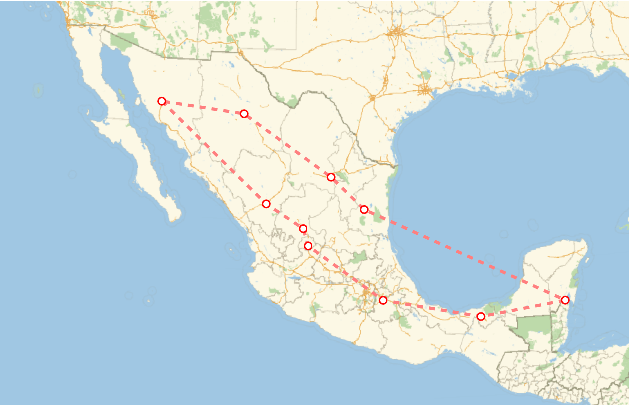
\includegraphics[scale=0.8]{../figures/trip_cities_10_bruteforce.pdf}
    \caption{Ruta óptima para 10 capitales mediante fuerza bruta.}
    \label{fig:bruteforce_path_cities_10}
\end{figure}

\begin{minted}[
    frame=none,
    autogobble,
    obeytabs=false,
    breaklines,
    tabsize=4,
    linenos=true,
    baselinestretch=1,
    firstnumber=last,
    bgcolor=bg!70,
    mathescape,
    numberblanklines=false
    ]{julia}
    julia> best, coords_per_iter, distance_per_iter = ts.simulated_annealing(init_guess, "geo"; init_temp=30, temp_factor=0.99, max_iter=1000);

    julia> map(x -> x.name, best)
    10-element Vector{String}:
    "chihuahua"
    "hermosillo"
    "durango"
    "zacatecas"
    "aguascalientes"
    "puebla"
    "villahermosa"
    "chetumal"
    "ciudadvictoria"
    "saltillo"

    julia> distance_per_iter[end]
    5416.112742134114
\end{minted}

Es interesante ver que la ruta óptima encontrada mediante el cómputo de todas las permutaciones y la ruta encontrada mediante el algoritmo de recocido simulado es la misma, con la diferencia en que la primera comienza en Hermosillo y la segunda en Chihuahua pero en realidad el recorrido es el mismo si se considera que debe ser redondo. Como la ruta es la misma, entonces el recorrido visual se verá igual que aquella mostrada en la \cref{fig:bruteforce_path_cities_10}.

Para terminar este trabajo se mostrará el recorrido óptimo encontrado para las 32 capitales de México (no se hizo la comparación con el método de fuerza bruta por las razones anteriormente mencionadas):
\begin{minted}[
    frame=none,
    autogobble,
    obeytabs=false,
    breaklines,
    tabsize=4,
    linenos=true,
    baselinestretch=1,
    firstnumber=last,
    bgcolor=bg!70,
    mathescape,
    numberblanklines=false
    ]{julia}
    julia> sample_cities = ts.sample_cities(32);

    julia> init_guess_indexes = ts.initial_guess(32);

    julia> init_guess = sample_cities[init_guess_indexes];

    julia> best, coords_per_iter, distance_per_iter = ts.simulated_annealing(init_guess, "geo"; init_temp=30, temp_factor=0.99, max_iter=1000);

    julia> map(x -> x.name, best)    # Recorrido de la ruta optima
    32-element Vector{String}:
    "toluca"
    "morelia"
    "queretaro"
    "guanajuato"
    "guadalajara"
    "aguascalientes"
    "zacatecas"
    "sanluispotosi"
    "ciudadvictoria"
    "monterrey"
    "saltillo"
    "durango"
    "chihuahua"
    "hermosillo"
    "mexicali"
    "lapaz"
    "culiacan"
    "tepic"
    "colima"
    "chilpancingo"
    "oaxaca"
    "tuxtla"
    "villahermosa"
    "chetumal"
    "merida"
    "campeche"
    "xalapa"
    "puebla"
    "tlaxcala"
    "pachuca"
    "cdmx"
    "cuernavaca"

    julia> distance_per_iter[end]    # Distancia de la ruta optima
    9161.352094270975
\end{minted}

La distancia que se obtiene al final del algoritmo permitiendo que se compute el número máximo de iteraciones es $9161.35\ km$, y la visualización de su respectivo recorrido se puede observar en la \cref{fig:trip_cities_32_sa}.
\begin{figure}[ht!]
    \centering
    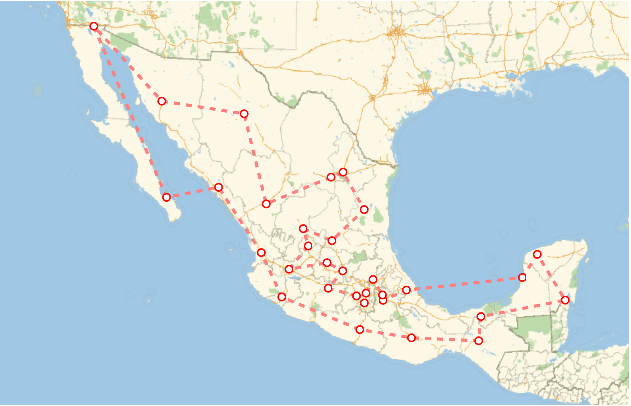
\includegraphics[scale=1.2]{../figures/trip_cities_32_sa.pdf}
    \caption{Ruta óptima para el recorrido de las 32 capitales de México.}
    \label{fig:trip_cities_32_sa}
\end{figure}

Antes de terminar este trabajo se quisiera aclarar un par de puntos importantes respecto a esta implementación:
\begin{itemize}
    \item Los caminos mostrados solamente reflejan las distancias que existen entre dos capitales no las rutas reales que se deberían de tomar. Si una persona pudiera viajar en \textit{línea recta}\footnote{Se abusó del significado de esta aseveración. Se hizo solamente con motivos ilustrativos.} sobre la superficie de una esféra cruzando los mares de manera indistinta entonces sí que sería la ruta que debería de recorrer.
    \item La distancia no es una distancia cartesiana como se acostumbra manejar en el mayor de los casos. Se usó una distancia computada mediante la fórmula de Haversine \cite{wiki2022haversine,movable2022haversine,stack2009haversine} la cual encuentra la distancia entre dos puntos en una esféra.
    \item El algoritmo utilizado en este trabajo fue adaptado de un código existente \cite{computational2021simulated}, se reescribió usando el lenguaje de programación \code{julia} y se adaptó para cumplir con los requisitos del proyecto.
    \item Las imágenes no se obtuvieron usando \code{julia}, para esto se exportaron las coordenadas de las rutas de cada imágen mostrada aquí y se procesaron con el lenguaje de programación \code{mathematica} el cual tiene funciones para graficar puntos en el mapa a partir de sus coordenadas.
\end{itemize}

Una idea para complementar este trabajo, la cual es más laboriosa ya que llevaría más tiempo de implementar, sería crear una matriz de adyacencia donde las entradas de dicha matriz fuesen las distancias de rutas reales entre ciudades. De esta manera ya no se necesitaría computar la distancia entre ciudades, estarían guardadas en una matriz y representarían realmente las distancias de carreteras dentro del país. Se tendría que definir una manera de acceder a la matriz a partir de un par de ciudades para buscar la distancia entre ellas, y la matriz sería una cuadrada de $32 \times 32$ debido al total de capitales.

\clearpage
\section*{Apéndice}
\inputminted[
    frame=none,
    autogobble,
    obeytabs=false,
    breaklines,
    tabsize=4,
    linenos=true,
    baselinestretch=1,
    firstnumber=1,
    bgcolor=bg!70,]{julia}{\codepath}

\nocite{*}    % to call all references even if they are not cited in the text
\bibliography{references.bib}

\end{document}

% \begin{minted}[
%     frame=none,
%     autogobble,
%     obeytabs=false,
%     breaklines,
%     tabsize=4,
%     linenos=true,
%     baselinestretch=1,
%     firstnumber=last,
%     bgcolor=bg!70,
%     mathescape,
%     numberblanklines=false
%     ]{julia}
%     # empty comment
% \end{minted}

